% ---------------------------------------------------------------- Task 1
\subsection{Task 1: the given hypotheses}

% ............................................................ H1
\subsubsection{H1 -- Longer time, higher score?}
\label{sec:h1}

\begin{hyp}{H1}
Students who take longer to complete the quiz tend to score higher.
\end{hyp}

\textbf{How we tested it.} We compared time taken with the grade, separately
for first attempts and for re-attempts, and separately for each quiz. Attempts
over 60 minutes were left out because they do not show real working time.

\textbf{Why this chart.} The grade has only six possible values and there are
more than 30,000 attempts, so a normal scatter plot would be a few solid
stripes of overlapping dots and would hide the pattern. Instead, for each grade
we show the \emph{median} time and the middle 50\% of times (IQR). This keeps
both the trend and the spread visible. We put first attempts and re-attempts
in two panels with the same y-axis (small multiples), so the two can be
compared directly.

\begin{figure}[H]
\centering
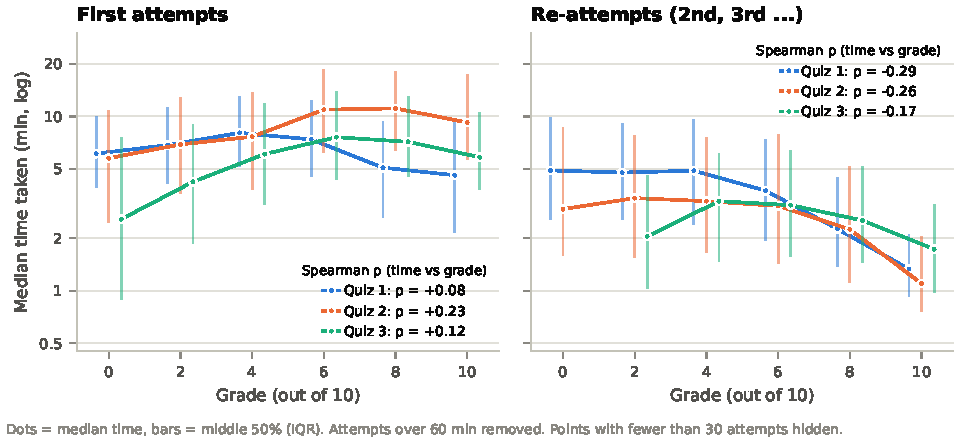
\includegraphics[width=\linewidth]{fig02_h1_time_vs_score.pdf}
\caption{H1. Median time taken (log scale) for each grade, with the
inter-quartile range. Left: first attempts. Right: re-attempts. Legends give
Spearman's $\rho$ between time and grade for each quiz.}
\label{fig:h1}
\end{figure}

\begin{mctable}
Median time per grade & Point & Vertical position (log) $\rightarrow$ median minutes; horizontal position $\rightarrow$ grade (ordered) \\
Spread & Line (vertical bar) & Length $\rightarrow$ inter-quartile range \\
Trend & Line connecting points & Slope $\rightarrow$ direction of change \\
Quiz & -- & Colour hue $\rightarrow$ quiz (categorical); small horizontal offset to avoid overlap \\
Attempt type & Separate panel & Spatial region $\rightarrow$ first vs.\ re-attempt \\
\end{mctable}

\textbf{What we see.} On \emph{first attempts} the lines go up from left to
right until about 6 or 8 marks: the median time rises from 6.0 minutes for a
grade of 0 to 8.5 minutes for a grade of 6. But the correlation is weak
(\rhoeq{0.08} for Quiz 1, 0.23 for Quiz 2 and 0.12 for Quiz 3), and students
with full marks were \emph{not} the slowest (6.5 minutes). On
\emph{re-attempts} the picture is reversed: the higher the grade, the shorter
the time, and a re-attempt with 10/10 took only about 1.3 minutes (\rhoeq{-0.17}
to $-0.29$). If we ignore the difference and put all attempts together, the
overall correlation becomes slightly negative (\rhoeq{-0.08}). This is a clear
case of Simpson's paradox: the two groups have opposite trends, and mixing them
hides both \citep{simpson1951interpretation}. The fast, high re-attempts are
explained in H7.

\begin{decision}
\textbf{Decision: \partly.} On a first attempt, taking longer goes with a
slightly higher score, but the link is weak ($\rho$ = 0.08--0.23) and it stops
at full marks. On re-attempts the opposite is true. So H1 is not true as a
general rule; it only holds weakly for first attempts.
\end{decision}

% ............................................................ H2
\subsubsection{H2 -- Are some questions consistently harder?}
\label{sec:h2}

\begin{hyp}{H2}
Some questions are consistently harder than others.
\end{hyp}

\textbf{How we tested it.} We measured difficulty with the facility index (\%
of first attempts that got the question right). ``Harder'' means a lower
facility index. ``Consistently'' needs a second check, so we tested whether the
same questions stay hard (i) for all three student tiers and (ii) across
the seven half-years in the data. We used first attempts only, because
re-attempts are affected by feedback.

\textbf{Why this chart.} Panel (a) is a heatmap because it gives a compact
overview of all 15 questions at once, with the exact value printed in each
cell, so readers do not have to judge colour alone. Panel (b) is a dot plot
because comparing tiers needs \emph{position on a common scale}, the most
accurate channel \citep{cleveland1984graphical}; the grey bar between the dots
shows the gap between Low and High students. Panel (c) is a second heatmap
with half-years as columns, so a stable ranking shows up as horizontal bands of
the same shade. Both heatmaps use the same sequential blue scale.

\begin{figure}[H]
\centering
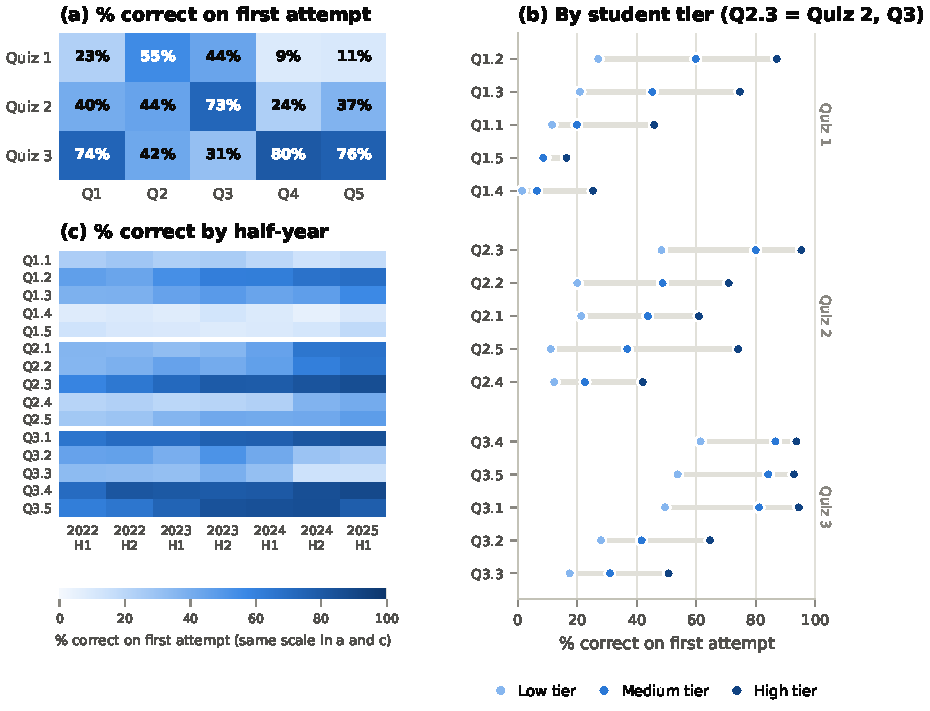
\includegraphics[width=\linewidth]{fig03_h2_question_difficulty.pdf}
\caption{H2. (a) Facility index (\% correct on first attempt) for each
question. (b) Facility by student tier; questions are sorted from easiest to
hardest within each quiz. (c) Facility for each half-year, same colour
scale as (a).}
\label{fig:h2}
\end{figure}

\begin{mctable}
(a), (c) cells & Area (rectangle) & Colour lightness (sequential blue) $\rightarrow$ \% correct; row/column position $\rightarrow$ quiz--question / half-year; text $\rightarrow$ exact value in (a) \\
(b) tier values & Point & Horizontal position $\rightarrow$ \% correct; vertical position $\rightarrow$ question; lightness of blue $\rightarrow$ tier (ordered) \\
(b) range & Line & Length $\rightarrow$ gap between tiers \\
\end{mctable}

\textbf{What we see.} The differences are large. Inside Quiz 1 the facility
goes from 55\% (Q1.2) down to 9\% (Q1.4) and 10\% (Q1.5). In Quiz 2 it goes
from 73\% (Q2.3) to 24\% (Q2.4), and in Quiz 3 from 80\% (Q3.4) to 31\%
(Q3.3). A chi-square test confirms that the questions inside each quiz are not
equally hard ($p < 0.001$, Cram\'er's $V$ = 0.33--0.41, a large effect).

The ranking is also stable. In panel (b), the hardest questions sit at the
bottom of their quiz for \emph{every} tier: even High-tier students get only
25\% of Q1.4 and 16\% of Q1.5 right, and Q3.3 is the hardest question in Quiz 3
for all three tiers. In panel (c) the rows keep their shade over time. The
hardest question in each quiz was the hardest in 6 of 7 half-years for Quiz 1
and in 7 of 7 for Quizzes 2 and 3. Kendall's $W$, which measures how much the
rankings agree across half-years, is 0.95, 0.85 and 0.87 (1 means perfect
agreement). Panel (c) also shows a few real changes, for example Q2.1 and Q2.2
became easier and Q3.2 and Q3.3 became harder in the second half of 2024. We
come back to this in H9.

\begin{decision}
\textbf{Decision: \accepted.} Some questions are much harder than others
(e.g.\ Q1.4 at 9\% vs.\ Q1.2 at 55\%), and the same questions stay hard for
weak and strong students and across three years.
\end{decision}

% ............................................................ H3
\subsubsection{H3 -- Do high performers improve steadily and low performers erratically?}
\label{sec:h3}

\begin{hyp}{H3}
High-performing students consistently improve scores over multiple attempts,
whereas low performers show erratic progress.
\end{hyp}

\textbf{How we tested it.} We took every student--quiz pair with at least two
attempts (8,130 pairs) and looked at how the grade changed from one attempt to
the next. We measured ``consistent improvement'' by the share of re-attempts
that went up, and ``erratic progress'' by the share of students (with three or
more attempts) whose grade dropped at least once.

There is a trap here. If tiers are defined using the same marks we are
studying, students put in the Low tier because of a bad first attempt will
improve partly by chance (regression to the mean, \citet{barnett2005regression}).
To check this, we repeated the analysis with a second tier definition that uses
\emph{only the other two quizzes} to decide a student's level.

\textbf{Why this chart.} Panel (a) is a line chart because attempt number is
ordered, and lines show the direction of change clearly; the shaded band is the
95\% confidence interval. Panel (b) uses 100\% stacked bars with a diverging
colour scale (red = down, grey = same, blue = up), so the share of each
direction can be read as a length and the ``bad'' and ``good'' sides are easy
to tell apart. Panel (c) uses dots with confidence intervals, and two shapes for
the two tier definitions, so the extra check sits right next to the main
result.

\begin{figure}[H]
\centering
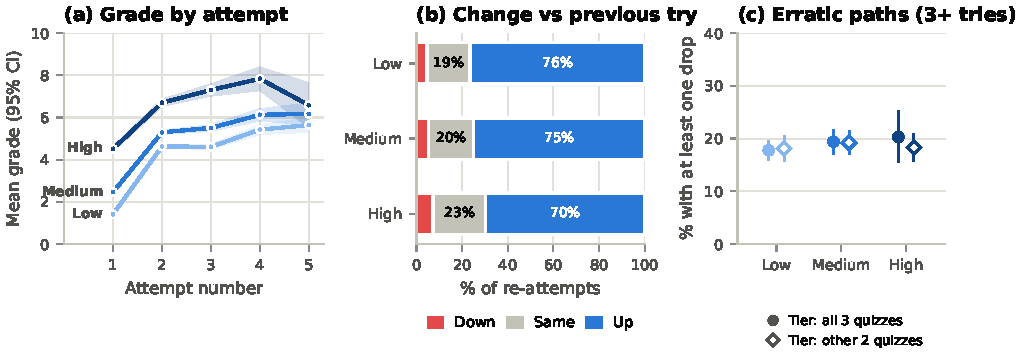
\includegraphics[width=\linewidth]{fig04_h3_progress_by_tier.pdf}
\caption{H3. (a) Mean grade by attempt number for each tier (students with 2+
attempts). (b) Direction of change from the previous attempt. (c) Share of
students with 3+ attempts whose grade dropped at least once; circles use the
normal tier, hollow diamonds use a tier based only on the other two quizzes.}
\label{fig:h3}
\end{figure}

\begin{mctable}
(a) mean grade & Point + line & Vertical position $\rightarrow$ mean grade; horizontal position $\rightarrow$ attempt number; lightness $\rightarrow$ tier \\
(a) uncertainty & Area & Band height $\rightarrow$ 95\% CI \\
(b) change & Line (bar segment) & Length $\rightarrow$ share of re-attempts; diverging hue $\rightarrow$ down / same / up \\
(c) erratic share & Point + error bar & Vertical position $\rightarrow$ \% with a drop; shape and fill $\rightarrow$ tier definition \\
\end{mctable}

\textbf{What we see.} All three tiers improve, and they improve in the same
way. In panel (b), 76\% of Low-tier re-attempts went up and only 5\% went down;
for High-tier students it was 70\% up and 7\% down. Low performers actually
gained the most from first to last attempt (+4.7 marks on average, against
+3.0 for High performers), because they started lower. Panel (c) shows that
``erratic'' paths are equally common in every tier: 18\% of Low, 19\% of Medium
and 20\% of High students with three or more attempts had at least one drop,
and the confidence intervals overlap. The hollow diamonds (tier from the other
two quizzes) give almost the same values (18\%, 19\%, 18\%), so the result is
not caused by regression to the mean.

The more useful explanation comes from H6: students mostly keep trying until
they pass and then stop, which makes almost everyone's path go up in the same
way.

\begin{decision}
\textbf{Decision: \rejected.} High performers do improve, but so do low
performers, and low performers are not more erratic. The share of drops is
about 5--7\% of re-attempts in every tier, and about 18--20\% of students with
3+ attempts in every tier.
\end{decision}

% ............................................................ H4
\subsubsection{H4 -- Do hard questions take longer, and are strong students faster on them?}
\label{sec:h4}

\begin{hyp}{H4}
More difficult questions take longer to answer, but higher-performing students
answer them faster than lower-performing students.
\end{hyp}

\textbf{An important limitation.} The data only gives the time for the
\emph{whole attempt}, not for each question. So this hypothesis cannot be
tested directly. We used two indirect tests instead.

\begin{enumerate}
  \item \textbf{Part 1, indirect test.} If a question needs more thinking time,
        then students who got it \emph{right} should have spent more time on the
        attempt than students who got it wrong, and this gap should be bigger
        for harder questions. For each of the 15 questions we calculated the
        ratio \emph{median time when correct $\div$ median time when wrong}
        (first attempts) and plotted it against the facility index.
  \item \textbf{Part 2, indirect test.} For the hardest question in each quiz,
        we took only the first attempts that got it right and compared the time
        taken by Low, Medium and High tier students.
\end{enumerate}

\textbf{Why this chart.} Part 1 compares two numeric values for 15 items, so a
labelled scatter plot is the natural choice; a horizontal reference line at 1
marks ``no time difference'' and a light trend line helps the eye. Part 2
compares a median between ordered groups, so we used dots with bootstrap
confidence intervals instead of bars, which would suggest a quantity that
starts from zero. Sample sizes are printed under each dot, because one group is
small.

\begin{figure}[H]
\centering
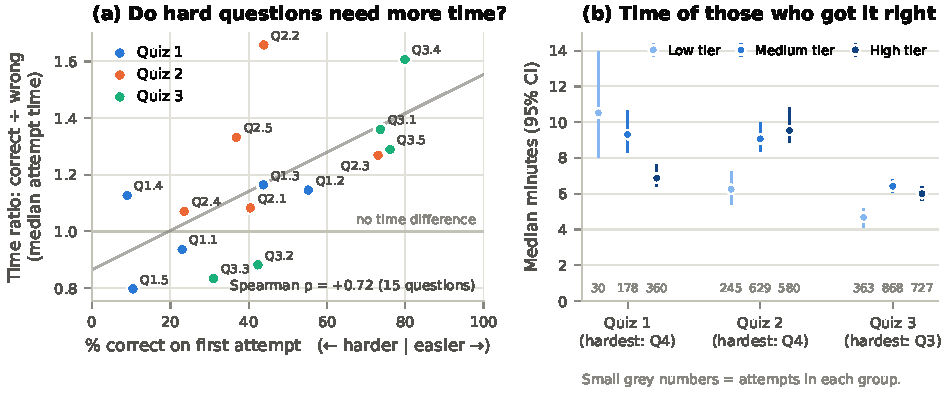
\includegraphics[width=\linewidth]{fig05_h4_difficulty_speed.pdf}
\caption{H4. (a) For each question: facility index vs.\ how much longer the
attempt took when the question was answered correctly. Points above 1 mean
correct answers came with more time. (b) Median time of first attempts that
answered the hardest question correctly, by tier, with 95\% bootstrap CIs.}
\label{fig:h4}
\end{figure}

\begin{mctable}
(a) question & Point & Horizontal position $\rightarrow$ facility index; vertical position $\rightarrow$ time ratio; hue $\rightarrow$ quiz; text $\rightarrow$ question ID \\
(a) reference & Line & Position $\rightarrow$ ratio of 1 (no difference) and linear trend \\
(b) tier medians & Point + error bar & Vertical position $\rightarrow$ median minutes; horizontal position $\rightarrow$ quiz and tier; lightness $\rightarrow$ tier \\
\end{mctable}

\textbf{What we see.} In panel (a) the points go \emph{up} to the right
(\rhoeq{+0.72}, $p = 0.003$). This is the opposite of Part 1: the time
``reward'' for getting a question right is biggest for \emph{easy} questions
(e.g.\ Q3.4 at 80\% facility, ratio 1.61) and smallest, or even below 1, for
hard ones (Q1.5 at 0.80, Q3.3 at 0.83). In other words, students who solve the
hardest questions do not seem to spend extra time on them. The quiz level gives
the same message: the hardest quiz (Quiz 1, mean 2.8/10) is not the slowest;
Quiz 2 is (median 8.4 minutes vs.\ 7.1 for Quiz 1).

Panel (b) supports Part 2 only in Quiz 1, where High-tier students who solved
Q1.4 needed 6.9 minutes against 9.3 for Medium and 10.5 for Low (but only 30
Low-tier students solved it). In Quiz 2 and Quiz 3 the result is reversed: the
Low tier was the \emph{fastest} (6.3 and 4.7 minutes). This matches a wider
pattern in the data: on first attempts, Low-tier students are the fastest in
all three quizzes (median 6.1, 6.3 and 5.1 minutes, against 7.3, 9.2 and 7.0
for the High tier). They seem to rush rather than to struggle.

\begin{decision}
\textbf{Decision: \rejected{} (with an important limitation).} Within what
the data allows us to test, hard questions do not go with longer times, and
higher-performing students are not generally faster; low performers are
usually the fastest. Because per-question times are not recorded, this is an
indirect test and the hypothesis should be re-checked with per-question time
logs.
\end{decision}

% ............................................................ H5
\subsubsection{H5 -- Is there an optimal time range?}
\label{sec:h5}

\begin{hyp}{H5}
There is an optimal time range for achieving higher scores, and students who
finish too quickly or take too long tend to score lower.
\end{hyp}

\textbf{How we tested it.} We grouped first attempts into time bins (from under
1 minute to over 1 day) and plotted the mean grade for each bin, per quiz. Here
we \emph{kept} the attempts over 60 minutes, because ``taking too long'' is part
of the hypothesis. We marked the best bin under one hour for each quiz.

\textbf{Why this chart.} An inverted-U shape is a question about the
\emph{shape} of a trend, which a line chart shows best. The x-axis is on a log
scale so that the short times, where most attempts are, get enough space. The
grey shaded area marks attempts over one hour, so readers know those times are
probably not real working time. The number of attempts per bin is shown in a
second, aligned panel instead of on a second y-axis, which would invite false
comparisons between the two scales.

\begin{figure}[H]
\centering
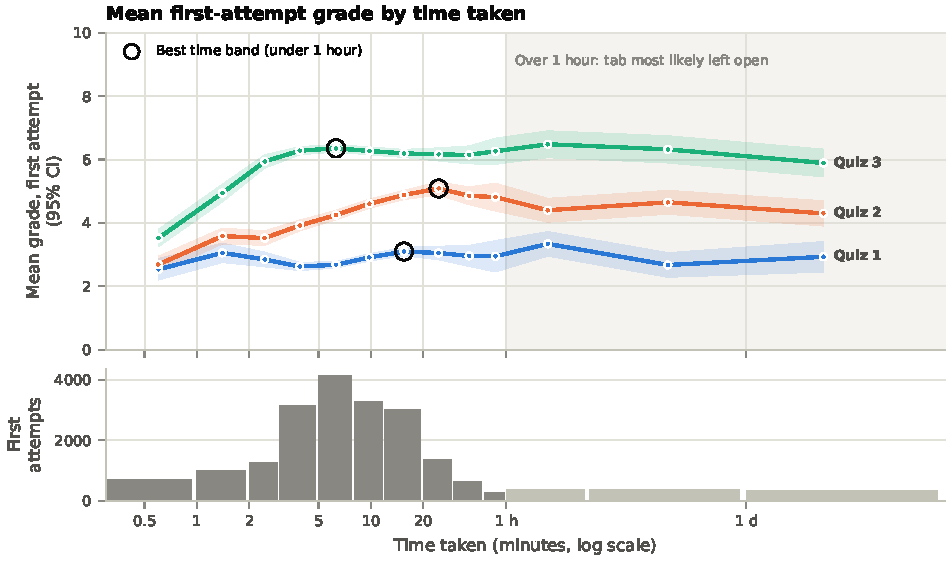
\includegraphics[width=\linewidth]{fig06_h5_optimal_time.pdf}
\caption{H5. Top: mean first-attempt grade by time bin with 95\% CI; circles
mark each quiz's best bin under one hour. Bottom: number of first attempts in
each bin. Bins: $<$1, 1--2, 2--3, 3--5, 5--8, 8--12, 12--20, 20--30, 30--45,
45--60 min, 1--3 h, 3--24 h, $>$1 day.}
\label{fig:h5}
\end{figure}

\begin{mctable}
Mean grade per bin & Point + line & Vertical position $\rightarrow$ mean grade; horizontal position (log) $\rightarrow$ time bin; hue $\rightarrow$ quiz \\
Uncertainty & Area & Band height $\rightarrow$ 95\% CI \\
Best bin & Point (ring) & Shape $\rightarrow$ ``best time band'' \\
Over 1 hour & Area (background) & Grey shade $\rightarrow$ probably idle time \\
Counts & Line (bar) & Length $\rightarrow$ number of attempts \\
\end{mctable}

\textbf{What we see.} The ``too fast'' part is very clear. First attempts
finished in under a minute score far lower: 2.5, 2.7 and 3.5 in Quizzes 1, 2
and 3, which is 1.6 marks below the quiz average when the quizzes are combined.
Scores rise quickly over the first few minutes and then level off. The best
band is different for each quiz: 5--8 minutes for Quiz 3 (6.35), 12--20 minutes
for Quiz 1 (3.10) and 20--30 minutes for Quiz 2 (5.09). After the peak the
lines go down only a little. Attempts left open for more than a day score
about the same as the quiz average (0.05 below), which is about 0.4 marks
below the peak. A simple curve fitted to all first attempts under an hour has
its peak at about 25 minutes. So there is a strong ``too fast'' penalty but
only a small ``too slow'' penalty, and the shape is more of a rise followed by a
plateau than a sharp peak. For Quiz 1, the hardest quiz, time hardly matters at
all.

\begin{decision}
\textbf{Decision: \partly.} Finishing too quickly clearly goes with lower
scores, and each quiz has a best time band. But taking too long has only a
small effect, so the ``inverted U'' is weak on the right side, and the best
band is not the same for every quiz.
\end{decision}
